% !TeX root = ../main.tex

\chapter{Numerical modelling method}


地球動力學為探討地球內部的動力過程,以及地球內部物質受力後所發生的變形作用,因此其所牽扯的運動狀態複雜,


地球動力學的研究主要涉及發生在地球表面以下的過程。地球上最深的鑽井資料為12公里(\citealp{ganchin1998seismic}),而地震學為目前最常見對地球深部構造的探勘方法。然而最早的地震學發展始於19世紀末,其所觀測得之構造在地質時間尺度上只能被視為瞬間狀態,無法代表地球內部過去的構造狀態。
地質學藉由地表觀察,可得知過去地表上經歷的地質事件,可間接獲得當時的動力狀態,不過隨著時間推移,可用的岩石紀錄越來越少,並且地質資料並無法有效代表地球內部的動力過程。
為了彌補地球動力學中有限的數據量,地質建模與模擬是探討地球內部演化常見的方法之一,例如沙箱模擬與計算機模型等。


在本研究的數值模型中,地球動力學所牽扯的運動過程複雜,不適用單純的質點或剛體運動,需要使用連續體力學(Continuum mechanics)的物理概念描述岩石的動力與變形行為。
在模型中將岩石單元視為地質構造上的連續介質(Continuum meduium),岩石具有巨觀物理量,受牛頓力學所支配,系統中的總力除了質點運動中所包含的外力(external force)之外,還需要考慮系統的內部作用力(internal force)。
連續介質特性描述可被用於岩石的密度、壓力、速度、應變等不同維度物理的場變量(field variables)。
由於在地質尺度上長期且緩慢的岩石變形過程可視為流體,因此地球動力學模型在不同尺度上部分可視為流體力學的展現。
而流體力學的數學式共有三大守恆定律,分別為質量守恆、動量守恆與能量守恆。
該三大守恆定律可寫成偏微分方程式的形式,同時也是連續方程式,此時因偏微分方程式之解析解多半不存在,僅能利用數值近似方法求得最佳解。

本研究的目的為探討平坦隱沒形成的條件以及演化發育過程。
在本章節中會先介紹數值模擬的計算方式以及模型中的假設,接著說明初始模型的設定。

\section{FLAC}

本研究使用Fast Lagrangian Analysis of Continua (FLAC,快速拉格朗日連續體分析) 技術,最早是由\citealp{cundall1989numerical}開發的二維顯性(explicit)有限差分(Finite Difference Method, FDM)數值分析軟體。
爾後由\citealp{Lavier2000}改良,適用於模擬地球動力與地球內部變形。
FLAC使用拉格朗日描述法(Lagrangian formulation)與非均值網格(structured non-uniform mesh),假設物質不可壓縮情況下並滿足boussinesq approximation求解主控方程式。
每個時間段上求解每個節點(node)的運動方程式,算出每個節點上所受到的力,計算出新的速度與位移,進而推算節點應變,再藉由岩石流變學物性方程式(constitutive equation)得到節點的應力,作為下一時間的初始作用力,流程見圖\ref{fig::FLAC_method}。

\begin{figure*}[ht!]
    \centering
    \includegraphics[width=4in]{FLAC_method.png}
    \caption{FLAC 程式運算流程圖
    }
    \label{fig::FLAC_method}
\end{figure*}

\section{主控方程式}

\subsection{質量守恆}

拉格朗日描述法的質量守恆方程式如下:

\begin{align}
\frac{\partial \sigma_{ij}}{\partial x_j}+\rho g_i = \rho \frac{\partial D_{vi}}{\partial t} 
\label{eqn:MASS_Lagrangian}
\end{align}

在本研究中,FLAC所使用的描述方法為拉格朗日描述法。
每個拉格朗日點被嚴格的連到一個單一的物質點上,並且會隨著該點移動。
因此,同一個質點總是在同一格座標上,與時間無關。

\begin{figure*}[ht!]
    \centering
    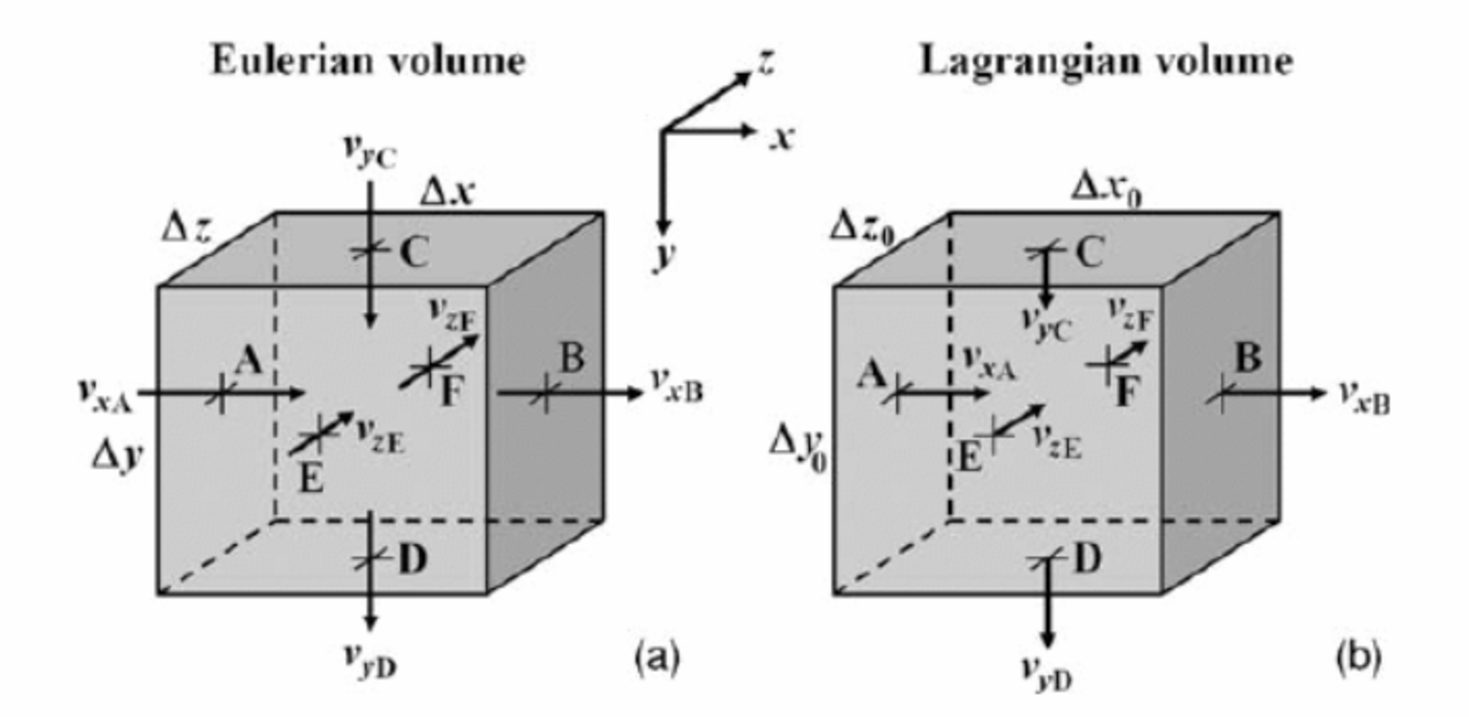
\includegraphics[width=4.5in]{eulerian_and_lagrangian.pdf}
    \caption{ Eulerian (a) and Lagrangian (b) elementary volumes considered for the derivation of continuity equation. }
    \label{fig::Lagrangian Volume}
\end{figure*}

式\ref{eqn:MASS_Lagrangian}的證明如下:

由於拉格朗日描述法中同樣的物質點永遠在相同的位置上,因此拉格朗日網格的質量永遠相同,但網格體積會因網格內在膨脹與收縮作用而隨時間改變。令一拉格往日網格體積為$V_0$,其初始平均密度$\rho_0$為:

\begin{align}
\rho_0 = \frac{m}{\Delta x_0 \Delta y_0 \Delta z_0}
\end{align}

經過一段短周期$\Delta t$時間後,受力之拉格朗日體積承受網格內內在作用,因此其體積變成$V_1$,而其平均密度$\rho_1$變成:
\begin{align}
\rho_1 = \frac{m}{\Delta x_1 \Delta y_1 \Delta z_1}
\end{align}
對拉格朗日流場所有自變數隨時間變化可表示為:
\begin{align}
\frac{D\rho}{Dt} \approx \frac{\Delta \rho}{\Delta t} = \frac{\rho_1-\rho_0}{\Delta t}=\frac{m}{\Delta x_1 \Delta y_1 \Delta z_1\Delta t}-\frac{m}{\Delta x_0 \Delta y_0 \Delta z_0\Delta t}\label{eqn:Drho-Dt}
\end{align}
在新舊拉格朗日體積中的關係可視為體積邊界的相對運動,由於位移等同於速度乘以持續時間:
\begin{align}
\Delta x_1 = \Delta x_0+\Delta t\Delta v_x\label{eqn:disx}\\ 
\Delta y_1 = \Delta y_0+\Delta t\Delta v_y\label{eqn:disy}\\
\Delta z_1 = \Delta z_0+\Delta t\Delta v_z\label{eqn:disz}
\end{align}
將上式 ($\ref{eqn:disx}$)-($\ref{eqn:disz}$)帶入(\ref{eqn:Drho-Dt})中可得:

\begin{align}
\frac{D\rho}{Dt} \approx \frac{\Delta \rho}{\Delta t} =\frac{m\Delta x_0 \Delta y_0 \Delta z_0-m\Delta x_1 \Delta y_1 \Delta z_1}{\Delta x_1 \Delta y_1 \Delta z_1\Delta t\Delta x_0 \Delta y_0 \Delta z_0}\label{eqn:Drho-Dt2}
\end{align}
由於$\Delta x_0 \Delta y_0 \Delta z_0=\rho_0$, 可獲得下列數學式:
\begin{align}
\frac{\Delta \rho}{\Delta t}+\rho_0\frac{\frac{\Delta v_x}{\Delta x_0}+\frac{\Delta v_y}{\Delta y_0}+\frac{\Delta v_z}{\Delta z_0}+K_1}{K_2} = 0
\end{align}
\begin{align}
K_1 = \Delta t(\frac{\Delta v_x}{\Delta x_0}\frac{\Delta v_y}{\Delta y_0}+\frac{\Delta v_x}{\Delta x_0}\frac{\Delta v_z}{\Delta z_0}+\frac{\Delta v_y}{\Delta y_0}\frac{\Delta v_z}{\Delta z_0}+\Delta t \frac{\Delta v_x}{\Delta x_0}\frac{\Delta v_y}{\Delta y_0}\frac{\Delta v_z}{\Delta z_0})
\end{align}
\begin{align}
K_2=(1+\Delta t\frac{\Delta v_x}{\Delta x_0})(1+\Delta t\frac{\Delta v_y}{\Delta y_0})(1+\Delta t\frac{\Delta v_z}{\Delta z_0})
\end{align}
其中$K_1$ 與 $K_2$ 係數在$\Delta t$趨近於$0$時分別為$0$與單位,因此可得:
\begin{align}
\frac{D\rho}{Dt}+\rho\frac{\partial v_x}{\partial x}+\rho\frac{\partial v_y}{\partial y}+\rho\frac{\partial v_z}{\partial z} = 0
\end{align}
或
\begin{align}
\frac{D\rho}{Dt}+\rho \nabla\cdot(\vec v) = 0 \label{eqn:Lagrangian continuity}
\end{align}

在數值模型中,主控方程式可以透過理想假設讓運算更為簡化,以下將介紹不可壓縮流(incompressible flow)與包辛尼斯克近似(Boussinesq approximation)。
不可壓縮流(incompressible flow)是一種簡化流體特性的物理假設,表示物質在流動時,密度不隨時間變化。
在一大氣壓下,移動中的物質若滿足馬赫數(Mach number,即流體速度與音速之比值。)小於0.3,則物質移動所造成的體積變化可忽略不計,此時不可壓縮流成立。
值得一提的是,地球內部的岩石承受極高壓力,彈性物質在靜止狀態下可能會在對抗壓力的同時體積縮小,密度變大,此時不可壓縮流假設並不成立。
因此如果要滿足不可壓縮流的假設,體彈性係數(Bulk modulus)需要遠大於壓力。
圖中顯示地球內部壓力與體彈性係數隨身度變化,在大約660公里深以上壓力與體彈性係數的比值夠大,可以視為不可壓縮流()。

在拉格朗日坐標系底下,密度變化等同體積變化,密度不改變等同體積不改變。可表示成:

\begin{align}
\frac{D\rho}{Dt} = 0 \label{eqn:imcompressible}
\end{align}

將$\ref{eqn:imcompressible}$帶入$\ref{eqn:Lagrangian continuity}$中得到:
\begin{align}
\rho \nabla\cdot(\vec v) = 0
\end{align}
因$\rho$ 不等於0,因此:
\begin{align}
\nabla\cdot(\vec v) = 0 \label{eqn:continuity final}
\end{align}


包辛尼斯克近似則是假設密度在所有運動方程式中皆為常數$\rho_0$,唯一無法近似的密度項是動量方程式中的浮力密度項。
該近似適用於密度變化不大的流體運動,因此通常是不可壓縮流。
需注意的是,在包辛尼斯克近似成立的情況下,絕熱溫度梯度(adiabatic temperature gradient)不存在,考慮絕熱溫度梯度存在時稱為廣義包辛尼斯克近似(extended Boussinesq approximation)。
在不可壓縮流中提及密度變化與體彈性係數有關,當體彈性係數為無限大,則彈性壓縮極小,密度變化趨近於零。
在等滳條件下體彈性係數的定義:
\begin{align}
K_S = -V(\frac{\partial P}{\partial V})_s = \rho(\frac{\partial P}{\partial \rho})_s
\end{align}
此時
\begin{align}
\frac{P}{K} = \frac{\Delta \rho}{\rho}
\end{align}


不可壓縮流假設與包辛尼斯克近似可以簡化主控方程式的密度項,將密度變化線性化:

\begin{align}
\rho (T) = \rho_0[1-\alpha (T-T_0)] 
\end{align}
其中 $\rho_0$ 是當溫度為$T_0$時的參考密度,$\alpha$是體積熱膨脹係數。

因此,所有三個主控方程式中只有動量守恆方程式會有二次項,其餘皆為線性方程式。
式$\ref{eqn:continuity final}$ 是本研究中所使用的質量守恆方程式。

\subsection{動量守恆}


% 我們所使用之運動方程式為Navier-Stokes equations,
地球內部的動力包含了介質所受之外力與內力力平衡的結果,並且在物質受力後產生變形。
在數值計算中利用動量守恆方程式將力與變形聯繫,使用牛頓第二運動定律。
\begin{align}
f=ma
\end{align}
$f$ 為作用在物質上的作用力,$m$為物質的質量。本研究所使用之拉格朗日坐標系下動量守恆方程式為:
\begin{align}
\frac{\partial \sigma_{ij}}{\partial x_j}+\rho g_i = \rho \frac{\partial D_{vi}}{\partial t}\label{eqn:momentum Lagrangian}
\end{align}
\begin{figure*}[ht!]
    \centering
    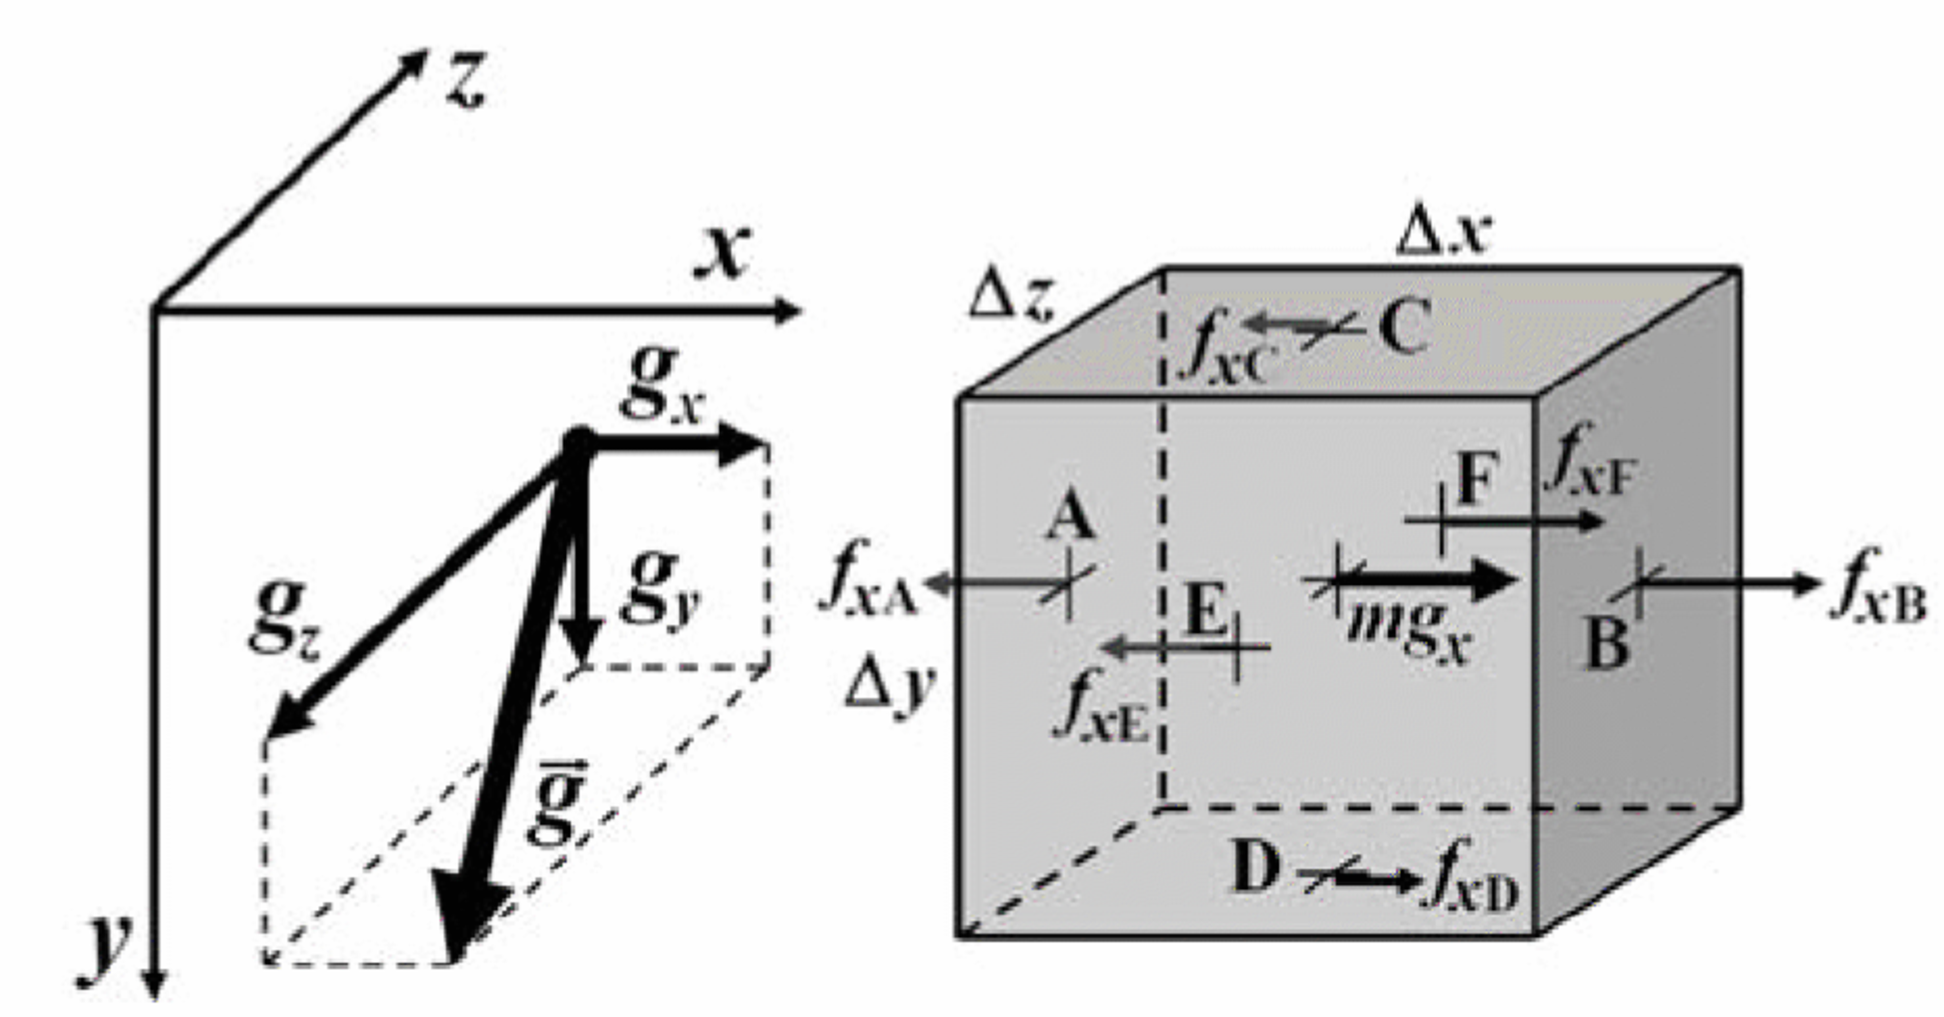
\includegraphics[width=4in]{momentum.pdf}
    \caption{ Lagrangian elementary Volume considered for the derivation of the respective form of x-momentum equation.}
    \label{fig::Lagrangian Volume Momentum}
\end{figure*}
利用計算作用於一小拉格朗日體積上之淨力(net forces)可證明$\ref{eqn:momentum Lagrangian}$:

對x分量而言,
\begin{align}
f_x=f_{xA}+f_{xB}+f_{xC}+f_{xD}+f_{xE}+f_{xF}+mg_x \label{eqn:Ftotal0}
\end{align}

$f_{xA}- f_{xF}$ 為與應力相關之力,其來自於各邊界A-F上體積外部。 
$f_g=m_gx$ 為重力。
% $f_{xA}- f_{xF}$ are stress-related forces, from the outside of the volume on the respective boundaries A-F. 
% $f_g=m_gx$ is the gravity force.
\begin{align}
f_{xA} = -\sigma_{xxA}\Delta y\Delta z\label{eqn:fxA}\\
f_{xB} = +\sigma_{xxB}\Delta y\Delta z\label{eqn:fxB}\\
f_{xC} = -\sigma_{xyC}\Delta x\Delta z\label{eqn:fxC}\\
f_{xD} = +\sigma_{xyD}\Delta x\Delta z\label{eqn:fxD}\\
f_{xE} = -\sigma_{xzE}\Delta x\Delta y\label{eqn:fxE}\\
f_{xF} = +\sigma_{xzF}\Delta x\Delta y\label{eqn:fxF}
\end{align}
將($\ref{eqn:fxA}$)-($\ref{eqn:fxF}$)帶入($\ref{eqn:Ftotal0}$)中得到:
\begin{align}
(\sigma_{xxB}-\sigma_{xxA})\Delta y\Delta z+(\sigma_{xyD}-\sigma_{xyC})\Delta x\Delta z+(\sigma_{xzF}-\sigma_{xzE})\Delta x\Delta y+mg_x = ma_x 
\end{align}
透過拉格朗日體積對左右兩式進行正交化:
\begin{align}
V=\Delta x\Delta y\Delta z
\end{align}
得到:
\begin{align}
\frac{(\sigma_{xxB}-\sigma_{xxA})\Delta y\Delta z}{V}+\frac{(\sigma_{xyD}-\sigma_{xyC})\Delta x\Delta z}{V}+\frac{(\sigma_{xzF}-\sigma_{xzE})\Delta x\Delta y}{V}+\frac{m}{V}g_x=\frac{m}{V}a_x
\end{align}
或
\begin{align}
\frac{\Delta\sigma_{xx}}{\Delta x}+\frac{\Delta\sigma_{xy}}{\Delta y}+\frac{\Delta\sigma_{xz}}{\Delta z}+\rho g_x = \rho a_x
\end{align}
當各個應力分量的差異趨近於零,可獲得
\begin{align}
\frac{\partial\sigma_{xx}}{\partial x}+\frac{\partial\sigma_{xy}}{\partial y}+\frac{\partial\sigma_{xz}}{\partial z}+\rho g_x = \rho a_x
\end{align}
或
\begin{align}
\partial_j\sigma_{ij}+\rho g_i = \rho \ddot u
\end{align}
其中 $u$ 是位移量。
\subsection{能量守恆}
為了描述一連續體中的能量平衡狀態,使用溫度方程式表示能量的進出。拉格朗日描述法下的能量守恆方程式表示如下:

\begin{align}
\rho C_p \frac{DT}{Dt} = -\frac{\partial q_x}{\partial x}-\frac{\partial q_y}{\partial y}-\frac{\partial q_z}{\partial z}+H_s+H_L
\end{align}

其中$\rho$是密度,$C_p$是等壓比熱容量,$H_s$是摩擦熱,$H_L$是潛熱。

因此在滿足包辛尼斯克近似的拉格朗日座標系下不可壓縮的能量守恆方程式為
\begin{align}
\nabla \cdot (\vec v) = 0 
\frac{\partial \sigma_{ij}}{\partial x_j}+\rho g_i = \rho \frac{\partial D_{vi}}{\partial t}
\rho C_p \frac{DT}{Dt} = -\frac{\partial q_x}{\partial x}-\frac{\partial q_y}{\partial y}-\frac{\partial q_z}{\partial z}+H_s+H_L
\end{align}

\section{岩石流變學}
主控方程式包含七個方程式與十個未知數,因此求解過程需要額外方程式。
岩石的流變學由物性方程式所表示,不同的岩石具有不同物理性質。

在近地表區域,岩石處於相對較低溫的環境,因此地球岩石圈表層由脆性變形(brittle deformation)所主導,包含低壓下的彈性變形(elastic deformation)與高壓下的塑性變形(plastic deformation)。
而在地球岩石圈深處到地球內部,岩石因周遭溫度隨深度增加而表現出不可逆的黏性變形(viscous deformation)。
因此,若地球動力學模型需同時考慮廣泛的岩石變形特性時,則模型流變學應同時包含彈-塑-黏性(elasto-visco-plastic)變形。

彈性流變假設物質所承受的應力與其應變呈正比,可以是虎克定律的展現。彈性變形很重要的精隨為其變形是可逆的,若施加在彈性物質上的應力被移除,其變形量會變回零。
由虎克定律得到彈性通式:

\begin{align}
\sigma_{ij}=C_{ijkl} 𝜀_{kl}
\end{align}
假設物質具有均質性(isotropic),則上列通式矩陣僅會有兩個獨立分量:

\begin{align}
    \sigma_{ij}=\lambda_1 ε_{kk} δ_{ij}+2 λ_2 ε_{ij}=Kε_{kk} δ_{ij}+2 \mu ε_{ij}^{dev} \label{eqn:elastic tensor}
\end{align}

彈性力學所使用的拉梅參數為$\lambda_1 = \lambda_2 = 3 \times 10^{10} Pa$,其中第一拉梅參數(Lamé's first parameter, $\lambda_1$)與體彈性系數(bulk modulus, $K$)、剪彈性系數(shear modulus, $\mu$)的關係式如下:

\begin{align}
\lambda_1 = K - \frac{2}{3}\mu
\end{align}

第二拉梅參數(Lamé's second parameter, $\lambda_2$)等同於剪彈性系數(shear modulus, $\mu$)。

本研究所使用的塑性變形滿足莫爾庫倫破壞準則(Mohr-Coulomb)定義屈服應力(yield stress)的大小:

\begin{align}
    \sigma_{yield}=C+tan(\phi)\sigma_{n}\label{eqn:plastic deformation}
\end{align}

其中$C$為內聚力,$\sigma_n$為正向力,$\phi$為物質摩擦角。
當破壞發生後,物質強度降低,發生應變弱化(strain weakening),其內聚力與摩擦角皆會降低。
本研究中假設破壞物質之內聚力與摩擦角會線性降低直到一飽和最小值,如圖\ref{fig::plastic_deformatiom},表示發生過破裂的區域強度變弱,使變形帶集中。
本研究各物質所使用的內聚力與摩擦角見表。
在應變率為$0$時,岩石摩擦角與內聚力分別為$C_0$, $\phi_0$ ; 在應變率大於$\varepsilon_(pl,saturate)$時,岩石摩擦角與內聚力分別為$C_1$, $\phi_1$ ; 當岩石應變率在0到$\varepsilon_(pl,saturate)$之間時,岩石摩擦角與內聚力的值會隨應變率在($C0$, $\phi0$)與($C1$, $\phi1$)之間線性遞減。
\begin{figure*}[ht!]
    \centering
    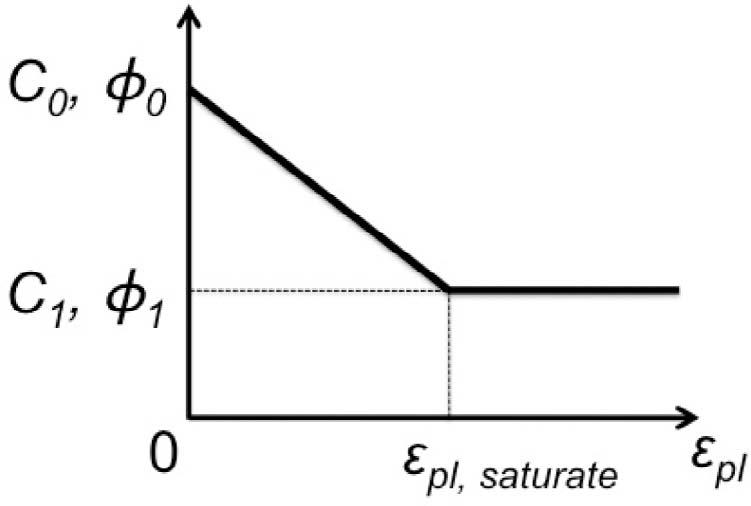
\includegraphics[width=3in]{Tan 2012 plastic.jpg}
    \caption{應力弱化示意圖,摘自\citealp{Tan2012}。岩石摩擦角與內聚力的值會隨應變率在($C_0$, $\phi_0$)與($C_1$, $\phi_1$)之間線性遞減。
    }
    \label{fig::plastic_deformatiom}
\end{figure*}

當溫度較高,材料強度相對進地表較低,以黏彈性(visco-elastic)變形為主。
本研究使用實驗結果所得的非牛頓流體位錯蠕變定律(dislocation creep laws)定義岩石黏滯度(\citealp{Chen1990}):

\begin{align}
   \eta=\frac{1}{4}(\frac{4}{3A})^{\frac{1}{n}} \dot\varepsilon_{II}^{\frac{1-n}{n}} exp(\frac{E}{nR(T+273)})
   \label{eqn:viscousity}
\end{align}
$\eta$為黏滯度,$\cdot\varepsilon$為應變率,$\cdot\varepsilon_{II}$為應變率張量矩陣的第二不變量,$n$為應力冪數(stress exponent),$A$為材料的指數前因子(viscosity pre-exponent),$T$為攝氏溫度,$E$為活化能(activation energy),$R$為氣體常數(universal gas constant)。
由於黏滯度會隨溫度升高而降低,本研究中,施加一臨界黏滯度最小值至$10^{20}\ Pa\cdot s$,以防止黏滯度過低導致計算量過大。
Gurnis et al. 2004已經表明臨界黏滯度為$10^{20}\ Pa\cdot s$足夠且不影響岩石圈動力學表現。
黏彈性應力與黏滯度、應變率成正比,其計算方式如下:	

\begin{align}
    \sigma_{vis} = 2\eta\dot\varepsilon \label{eqn:viscous tensor}
\end{align}
在同一網格中會分別計算黏彈性應力與
計算每個網格上的$\sigma_{plastic}$與$\sigma_{viscous}$,最終每個網格所採計的應力值為($\sigma_{elasto-plastic}$, $\sigma_{elasto-viscous}$)兩者之間的最小值。
\section{相變}

為了模擬自然界中岩石動力學中的物理性質變化,本研究考慮部分岩石相變機制,利用岩石溫度壓力狀態當作簡單相變條件。
考量相變過程可以讓隱沒模型之運動況狀以更真實的型態呈現,更能真實展現隱沒帶中力學分配過程。

在本研究中,使用模型中的標記點追蹤物質之岩相與位置,一旦所在網格之溫度與壓力滿足標記點物質之相變條件,則會判定該標記點發生相變,其岩相轉換為相變後之新岩相。
相變完成後,標記點物質所有物理性質皆會從原先岩相之性質轉變成新岩相之性質。
由於相變過程不影響運動狀態,但與溫度相關,因此嗎行中在考慮相變時,該位置溫度會將絕熱溫度梯度加回模型的溫度中。
以下將一一列出模型中所考慮的相變過程:

\subsection{Peridotite --- Serpentinite}
橄欖岩---蛇紋岩
一旦隱沒板塊進入地函中,隱沒海洋板塊上之沉積物在高溫高壓下會釋放大量流體至楔中,絕大部分集中在mantle wedge。乾的地函楔因而經歷水合作用,導致部分橄欖岩被蛇紋岩化。
蛇紋岩化橄欖岩主要集中於隱沒帶中淺部,並且目前人類對於蛇紋岩化橄欖岩之相變作用尚未有高度不確定性,因此本研究中以參數化方式模擬蛇紋岩化橄欖岩相變過程。
使用者可自行調整在隱沒板塊上方有多少厚度的地函楔會因脫水作用相變成蛇紋岩化橄欖岩(\citealp{Tan2012})。
在本研究中,蛇紋岩化之橄欖岩岩相物理性質約略等同於橄欖岩中有百分之15之橄欖岩被蛇紋岩化,其活化能大幅減少。
   
蛇紋岩化橄欖岩將隱沒帶流體帶入更深的地函中後,約在80-120公里之間再次發生脫水將水分釋放至地函楔中。
在本研究中,在符合以下溫壓條件時(\citealp{Ulmer1995}),該脫水作用成立,蛇紋岩化橄欖岩將相變回橄欖岩:
\begin{align}
T> 550 ^{\circ}\\
P > 2.1 GPa
\end{align}

圖為橄欖岩相溫壓相圖。

\subsection{Basalt --- Eclogite}

隨著隱沒板塊沉入更深的地函,其上的鎂鐵質玄武岩在高壓條件下進入榴輝岩穩定場,此時發生玄武岩相變,由高溫高壓實驗可獲得穩定場溫壓界線(\citealp{Hacker2003}),詳見下圖鎂鐵質岩相圖\ref{fig::basalt_phase_diagram}。
榴輝岩在隱沒帶中扮演非常重要的角色,同第一章所提及,榴輝岩是變質岩相中密度最大的相,造成的重力效應可以維持隱沒帶的持續性,是板塊移動的驅動力。
在該模型中,網格內的標記子會追蹤玄武岩海洋地殼的溫壓狀態,並與榴輝岩穩定性場進行了比較,以下方程為鎂鐵質玄武岩相變的簡化條件式。

\begin{align}
    P > 0.0022 \times T -0.3  \quad GPa\\
    P > -0.0375 \times T + 20.1  \quad GPa
\end{align}

\begin{figure*}[ht!]
    \centering
    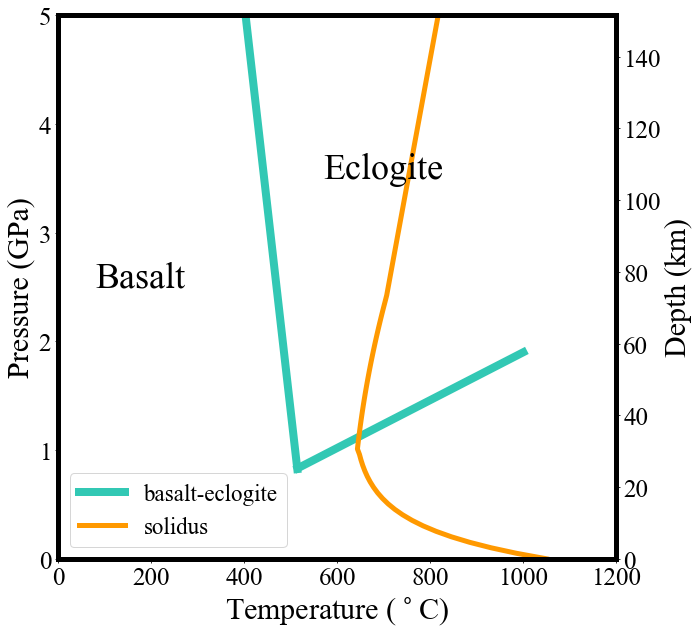
\includegraphics[width=3in]{basalt_phase_diagram.png}
    \caption{鎂鐵質岩相圖,綠線隔開玄武岩與榴輝岩的穩定場,改編自\citealp{Hacker2003},橘線為鎂鐵質岩的濕固相線(wet solidus),改編自\citealp{Gutscher2000Bcan}}
    \label{fig::basalt_phase_diagram}
\end{figure*}

\subsection{Sediment --- Schist}
模型中的沈積物在隱沒過程中進入高壓環境,發生成岩作用、壓密作用與變質作用。
不過由於這一系列作用是連續的,因此模型中的相變過程並不會造成岩石有大幅度物理性質上的改變。
下列方程為沈積物轉為片岩過程的條件式。
\begin{align}
T > 650^{\circ} C\\
depth >  20  \quad km 
\end{align}
本研究有考量沈積物的部分熔融,參考自\citealp{Forster2021}與圖\ref{fig::sediment_phase_diagram.png}。
\begin{align}
    T > max (578+ P \times 0.121, 617+e^{P\times 1.7\times 10^{-3}})
\end{align}

\begin{figure*}[ht!]
    \centering
    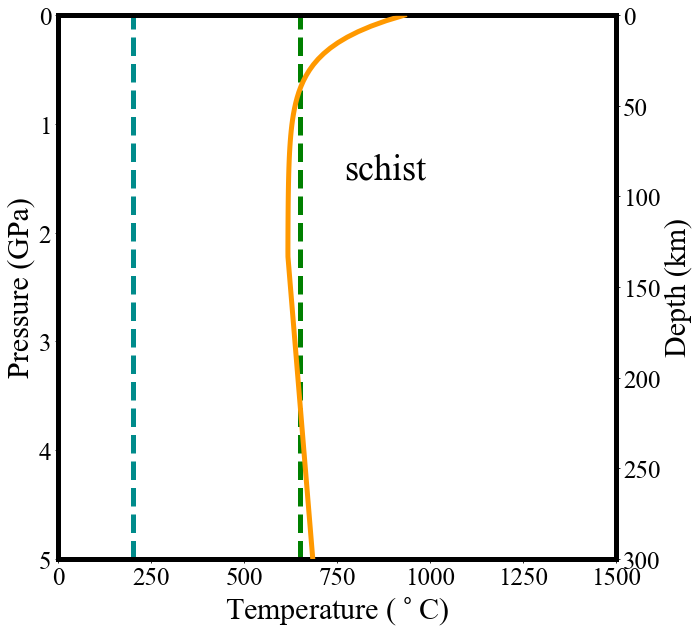
\includegraphics[width=3in]{sediment_phase_diagram.png}
    \caption{沈積物變質岩相圖,橘線為沈積物濕固相線,改編自\citealp{Forster2021}。}
    \label{fig::sediment_phase_diagram.png}
\end{figure*}


\subsection{Hydrated olivine --- Peridotite}

模型中的地函除了普通橄欖岩與蛇紋岩之外,還有考慮含水的橄欖岩。
本研究假設只有在含水橄欖岩上方的地函楔會發生部分熔融事件。
一旦溫度太高而使岩石脫水,含水橄欖石就會轉變為一般的橄欖岩。
相變條件式與相圖()如下。

\begin{align}
T > 800-35\times 10^{-9}\times (depth-62)^{2\circ}C
\end{align}

\section{邊界條件}

\subsection{運動邊界條件}
在現實自然界中,板塊隱沒主要由ridge push和slab pull兩個力作用所引起水平移動,而在數值模型中,主要驅動板塊隱沒的力由邊界條件速度所控制。於本研究中所使用的板塊水平移動運動起初由運動邊界條件所決定。然而,板塊移動速度與時間的關係不應為常數,於是在模型進行一段時間後,讓模型邊界條件隨邊界所承受之總體力大小所決定。

模型會先設定左右邊界最大可施加的力臨界值大小Fc,當模型進行一萬個迴圈後,若邊界承受的力大於初始所給定的力臨界值,則會將速度下降為原先的0.9倍;反之若邊界承受的力尚未達到給定的力臨界值,則速度會增加為原先的1.1倍。此時,每一萬個迴圈,模型運動邊界條件會重新調整一次,以符合觀測結果。因此當模型運行一段時間之後,邊界所承受的力會約略相等於初始條件所設定的力臨界值。

\subsection{熱邊界條件}
本研究中海洋岩石圈溫度構造使用半空間冷卻模型(half space cooling model),海洋岩石圈厚度與岩石圈年紀之開根號呈正比。由 \citealp{davis1974}提出:
\begin{align}
T=T_m\cdot {erf}(\frac{z}{2\sqrt{\kappa t}})
\end{align}
$T$ 是溫度,$T_m$ 是地函溫度,在本研究中使用1603K。
$z$ 是與地表的距離,單位是公里,$\kappa$ 是熱擴散系數,在本研究中使用$10^{-6}$。$t$ 是海洋岩石圈年紀,單位是秒。

大陸板塊的溫度構造有雙層構造與單層構造之區別。在靠近海溝的大陸岩石圈為雙層構造,近地表每公里20度溫度梯度,到45公里深之後溫度梯度為每公里6度,此溫度條件建立在Meana et al., 2005墨西哥區域溫度模型。遠離海溝測的大陸地溫梯度則是單層構造,以岩石圈底部深度作為參考,從地表0度到岩石圈底部1330度中間進行線性內插,僅含單一地溫梯度。不同構造區溫度隨深度變化圖見圖2-2。熱量傳遞在岩石圈以傳導為主,溫度變化極大,然而在軟流圈,熱量傳遞以對流為主,因此整個軟流圈至地幔地核邊界(core mantle boundary)的溫度皆維持地幔絕熱溫度,僅存在因密度變化所造成之溫度梯度,因此模型中將岩石圈底部溫度固定為地幔絕熱溫度1330度。

\section{地表侵蝕}
地表地形演化與板塊構造活動有高度相關,在本研究模型中利用較簡單的方式模擬地形演化過程,包含侵蝕與沈積物堆積作用,使用一維擴散方程式控制侵蝕與堆積作用的速率,最早由\citealp{culling1960analytical} 所提出,其方程式如下:

\begin{align}
\frac{\partial z}{\partial t} = \kappa \nabla^2 z \label{eq: erosion}
\end{align}

其中$z$為模型中地表節點高度,其數學意義為對地表高度進行二次導數後得到該點曲率,並照曲率大小對其進行地形下修與上修,地形較突出處會被侵蝕,反之地形凹陷處容易被侵蝕物所堆積。物理意義則為守恆公式之展現,將地形假想為一二維空間方程式,在地形上每一點會因重力而有往下流動物質通量S,流動物質通量與地形坡度呈正比:
\begin{align}
S = -k\nabla z \label{eq: S}
\end{align}
其中$k$為正比係數。並且由於物質永遠守恆,在滿足守恆公式的假設下,物質質量不隨時間變化,令物質質量與時間的關係式:
\begin{align}
\rho\frac{\partial z}{\partial t}\label{eq:rho}
\end{align}

質量隨時間的變化會等同於物質在空間中的通量,因此式($\ref{eq: S}$) 與式($\ref{eq:rho}$) 的關係如下:q 

\begin{align}
\rho\frac{\partial z}{\partial t} = -\vec\nabla\cdot \vec S = -\vec\nabla \cdot (-k\nabla z)\label{eq:erosion2}
\end{align}
或
\begin{align}
\frac{\partial z}{\partial t} = \frac{k}{\rho}\nabla^2 z\label{eq:erosion3}
\end{align}
令$\frac{k}{\rho}=\kappa$,其中$\kappa$為坡度擴散係數,本研究中侵蝕與堆積的坡度擴散係數相同,單位為$\frac{m^2}{s}$。可得:
\begin{align}
\frac{\partial z}{\partial t} = \kappa\nabla^2 z\label{eq:erosion4}
\end{align}

\section{岩漿作用}
本研究中,數值模型包含隱沒帶中的岩漿作用。
隱沒板塊進入地函時,其上的沈積物與玄武岩在進入高溫高壓環境的同時發生脫水與相變。
水分進入地函楔中,導致隱沒板塊上方的橄欖岩融點大幅降低,此時橄欖岩容易經過含水固相線(solidus)。
\subsection{部分熔融}
本研究共考慮三種成分的部分熔融,分別為在地函楔中的橄欖岩相(包含橄欖岩與蛇紋岩)、沈積岩相與鐵鎂質岩相(包含玄武岩與榴輝岩)。
模型中容許多個部分熔融事件發生。

\subsection{岩漿庫}
模型中假設有$F_M$比例的岩漿留在地函楔中,$F_C$比例的岩漿留在地殼中,其餘百分之$1-F_M-F_C$的岩漿會噴發至地表,使用可自行調整百分比。
部分熔融發生後,從熔融點開始產生一倒三角形的岩漿庫,岩漿庫頂部為在莫合面下,並在莫合面處達到最大寬度$M_W$公里。
岩漿庫中每個網格的體積融化比例(M)為與時間相關的函數,每次的部分熔融事件所產生的岩漿會在模型中累積。每個時間點的體積融化比例分為每個時間點產生的岩漿量與每個時間點冷卻的岩漿量,由下式表示:
\begin{align}
    M(t+dt)-M(t) = \Delta M = Pdt-M(t)\lambda dt \label{eq:Magma}
\end{align}
\begin{align}
    P = P_0 \times pmelt \times F_M \times A
\end{align}
\begin{align}
    \lambda = \lambda_0 exp(-\lambda_T\Delta T)
\end{align}
其中$P$為岩漿產生速率,$P_0$是模型可調整的參數,單位為$m^2/s$,$pmelt$為部分熔融百分比,$A$為發生部分熔融的面積。
$\lambda_0$為岩漿冷卻無單位常數,$\lambda_T$是與溫度有關的冷卻係數,單位為$\frac{1}{K}$。

\subsection{岩漿作用造成的溫度影響}
在岩漿冷卻的過程中,會釋放潛熱,導致週遭岩石的溫度有局部升高的現象。模型中會計算每個時間的岩漿變化量($\Delta M$),計算溫度變化量,使用公式如下:
\begin{align}
    T(t+dt) = T(t) + \frac{\Delta M L_H}{C_P}\label{eq:latent heat}
\end{align}
其中$L_H$為岩漿潛熱值,載本研究中使用安山岩漿的潛熱值$3.5\times 10^5$ J/m()。$C_P$為熱容。